\documentclass[11pt]{article}
\usepackage{graphicx}
\usepackage[tmargin=1in,bmargin=1in,lmargin=1in,rmargin=1in]{geometry}
\usepackage{pdfpages}
\usepackage{parskip}
\usepackage{mypackagesv2}
\usepackage{caption}
\graphicspath{ {images/} }

\title{Design Calculations} 
\author{Jadon Tsai $|$ Jeffery Tian $|$ Pranav Upreti}
\everymath{\displaystyle}

\begin{document}
\maketitle
\tableofcontents
\newpage

\section{Hand Calculations}
Below are our hand calculations for the factors of safety against failure for Design 0 and hand calculations for the factors of safety.

\subsection{Design 0}
The hand calculations to determine the Factor of Safety for each potential cause of failure are shown below. Note that we used values taken from our code for some of our calculations. However, the last two pages are hand calculations verifying the values from our code. The train was assumed to be moving, but with a load configuration that can be seen below in Figure 1.
\begin{figure}[H]
\centering
\begin{tikzpicture}
    % define coordinates
    \point{start}{0}{0};
    \point{end}{12}{0};
    % load coordinates;
    \point{l1}{1.72}{0};
    \point{l2}{3.48}{0};
    \point{l3}{5.12}{0};
    \point{l4}{6.88}{0};
    \point{l5}{8.52}{0};
    \point{l6}{10.28}{0};
    % specify beam location;
    \beam{2}{start}{end}[1][1];
    % specify support locations;
    \support{1}{start} % pin;
    \support{2}{end} % roller;
    % specify point loads;
    \load{1}{l1}[90];
    \load{1}{l2}[90];
    \load{1}{l3}[90];
    \load{1}{l4}[90];
    \load{1}{l5}[90];
    \load{1}{l6}[90];
    % label point loads;
    \notation{1}{l1}{66.7 KN}[above=12.5mm];
    \notation{1}{l2}{66.7 KN}[above=12.5mm];
    \notation{1}{l3}{66.7 KN}[above=12.5mm];
    \notation{1}{l4}{66.7 KN}[above=12.5mm];
    \notation{1}{l5}{66.7 KN}[above=12.5mm];
    \notation{1}{l6}{66.7 KN}[above=12.5mm];
    % dimension beam;
    \dimensioning{1}{start}{l1}{-1.45}[172 mm];
    \dimensioning{1}{l1}{l2}{-1.45}[176 mm];
    \dimensioning{1}{l2}{l3}{-1.45}[164 mm];
    \dimensioning{1}{l3}{l4}{-1.45}[176 mm];
    \dimensioning{1}{l4}{l5}{-1.45}[164 mm];
    \dimensioning{1}{l5}{l6}{-1.45}[176 mm];
    \dimensioning{1}{l6}{end}{-1.45}[172 mm];
\end{tikzpicture}
\caption{Base case loading diagram for load case 1}
\label{fig:load_case_1}
\end{figure}
From our calculations, we discovered that the center of the top flange of Design 0 would fail in Case 1 local buckling, with a Factor of Safety against failure of $\fbox{0.704}$.
\begin{figure}[H]
    \centering
    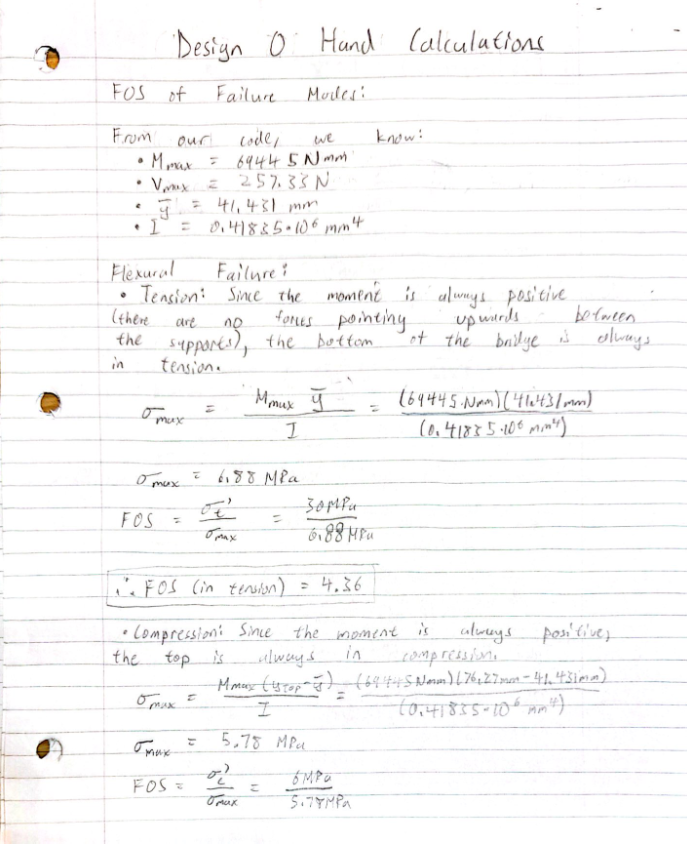
\includegraphics[width=0.95\linewidth]{images/D0 Hand Calcs P1.png}
\end{figure}
\begin{figure}[H]
    \centering
    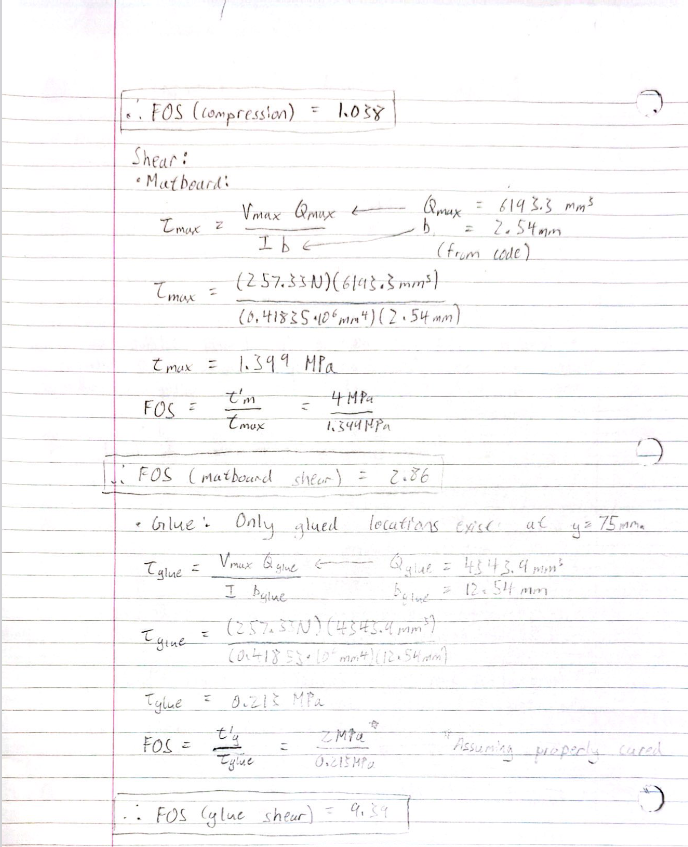
\includegraphics[width=0.95\linewidth]{images/D0 Hand Calcs P2.png}
\end{figure}

\begin{figure}[H]
    \centering
    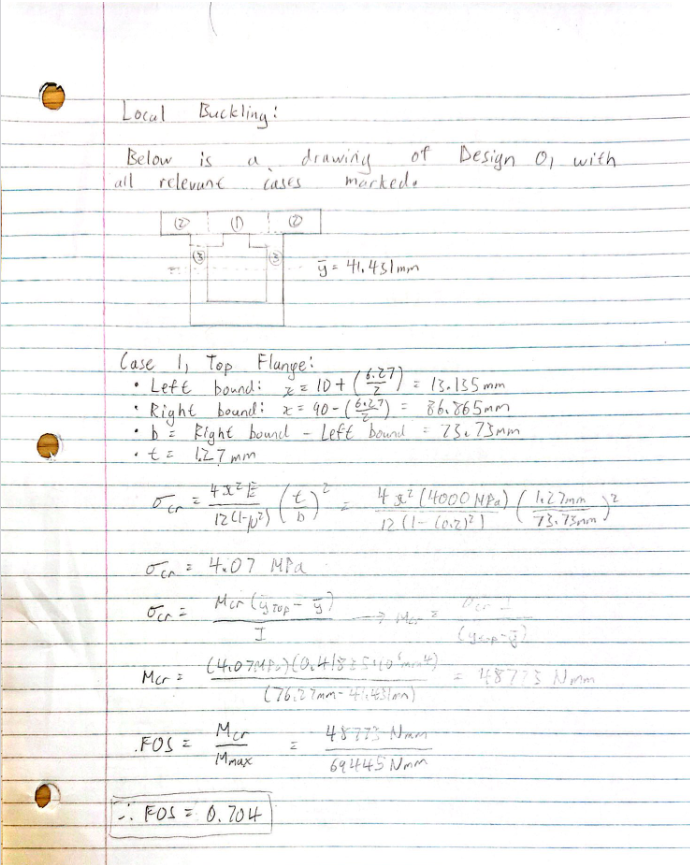
\includegraphics[width=0.95\linewidth]{images/D0 Hand Calcs P3.png}
\end{figure}

\begin{figure}[H]
    \centering
    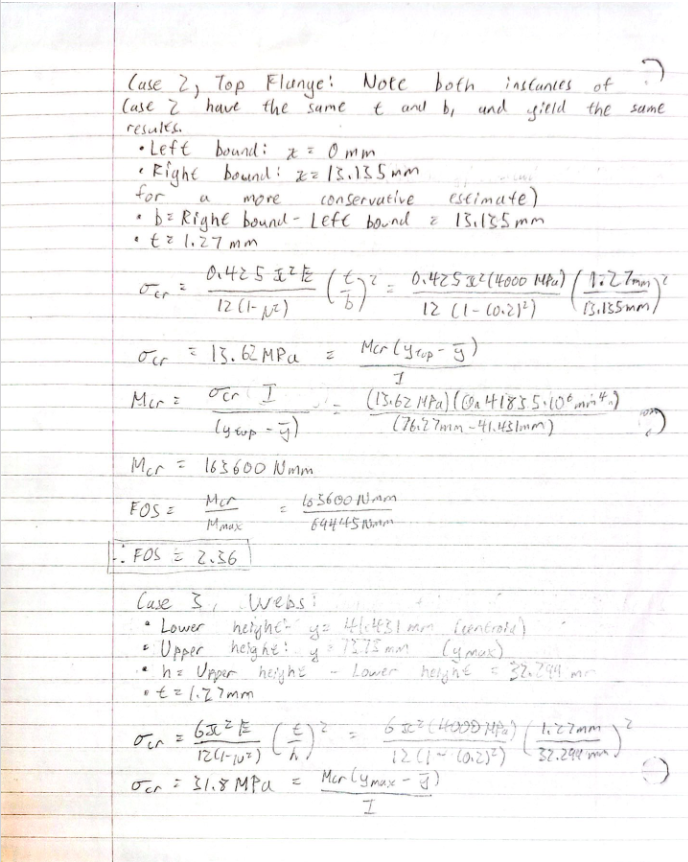
\includegraphics[width=0.95\linewidth]{images/D0 Hand Calcs P4.png}
\end{figure}

\begin{figure}[H]
    \centering
    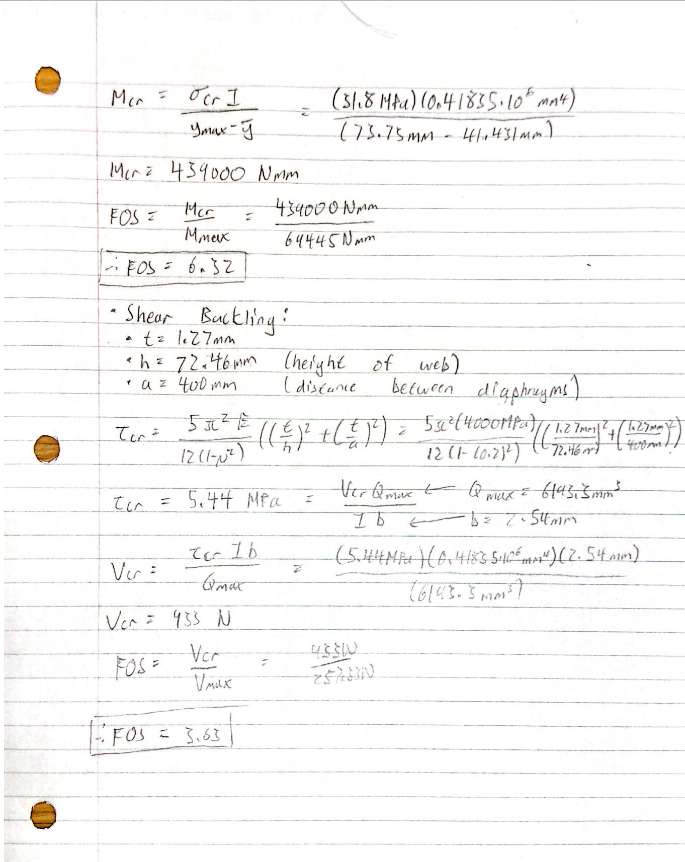
\includegraphics[width=0.95\linewidth]{images/D0 Hand Calcs P5.png}
\end{figure}

\begin{figure}[H]
    \centering
    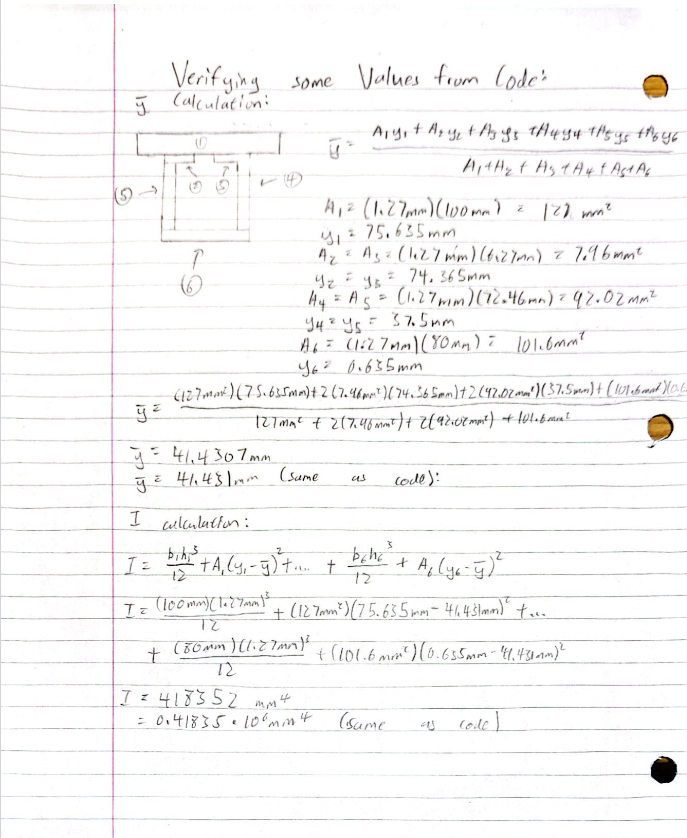
\includegraphics[width=0.95\linewidth]{images/VerifyingCode.png}
\end{figure}

\begin{figure}[H]
    \centering
    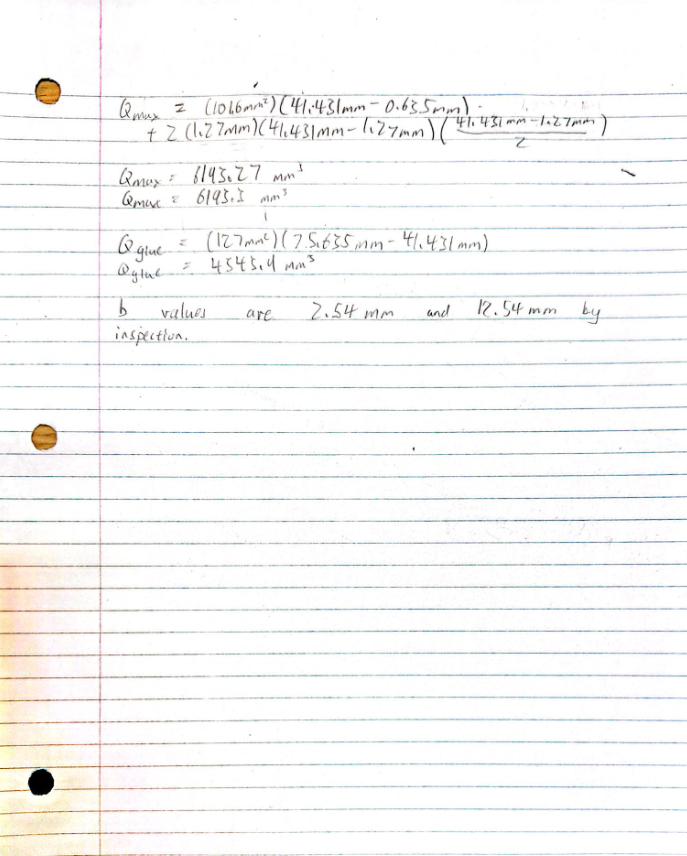
\includegraphics[width=0.95\linewidth]{images/VerifyingCodeP2.png}
\end{figure}
\subsection{Factors of Safety for our Bridge Design}
Though most of our values were generated using our Python script, we performed calculations by hand to determine our design's final factors of safety against each potential case of failure, both for the originally designed cross-section and along our splice connection.
\begin{figure}[H]
\centering
\begin{tikzpicture}
    % define coordinates
    \point{start}{0}{0};
    \point{end}{12}{0};
    % load coordinates;
    \point{l1}{1.72}{0};
    \point{l2}{3.48}{0};
    \point{l3}{5.12}{0};
    \point{l4}{6.88}{0};
    \point{l5}{8.52}{0};
    \point{l6}{10.28}{0};
    % specify beam location;
    \beam{2}{start}{end}[1][1];
    % specify support locations;
    \support{1}{start} % pin;
    \support{2}{end} % roller;
    % specify point loads;
    \load{1}{l1}[90];
    \load{1}{l2}[90];
    \load{1}{l3}[90];
    \load{1}{l4}[90];
    \load{1}{l5}[90];
    \load{1}{l6}[90];
    % label point loads;
    \notation{1}{l1}{67.5 KN}[above=12.5mm];
    \notation{1}{l2}{67.5 KN}[above=12.5mm];
    \notation{1}{l3}{67.5 KN}[above=12.5mm];
    \notation{1}{l4}{67.5 KN}[above=12.5mm];
    \notation{1}{l5}{91 KN}[above=12.5mm];
    \notation{1}{l6}{91 KN}[above=12.5mm];
    % dimension beam;
    \dimensioning{1}{start}{l1}{-1.45}[172 mm];
    \dimensioning{1}{l1}{l2}{-1.45}[176 mm];
    \dimensioning{1}{l2}{l3}{-1.45}[164 mm];
    \dimensioning{1}{l3}{l4}{-1.45}[176 mm];
    \dimensioning{1}{l4}{l5}{-1.45}[164 mm];
    \dimensioning{1}{l5}{l6}{-1.45}[176 mm];
    \dimensioning{1}{l6}{end}{-1.45}[172 mm];
\end{tikzpicture}
\caption{Base case loading diagram for load case 2}
\label{fig:load_case_2}
\end{figure}
We used the cross-section shown below, with hand calculations on the page following.
\begin{figure}[H]
    \centering
    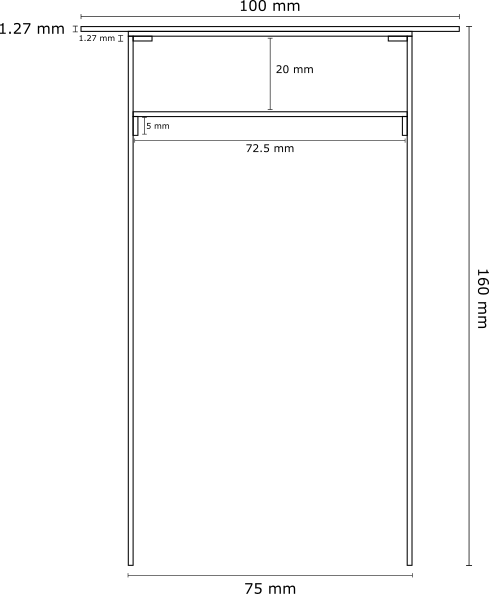
\includegraphics[width=0.8\linewidth]{rect238.png}
    \caption{The cross-section we used to build the bridge drawn to scale. }
\end{figure}
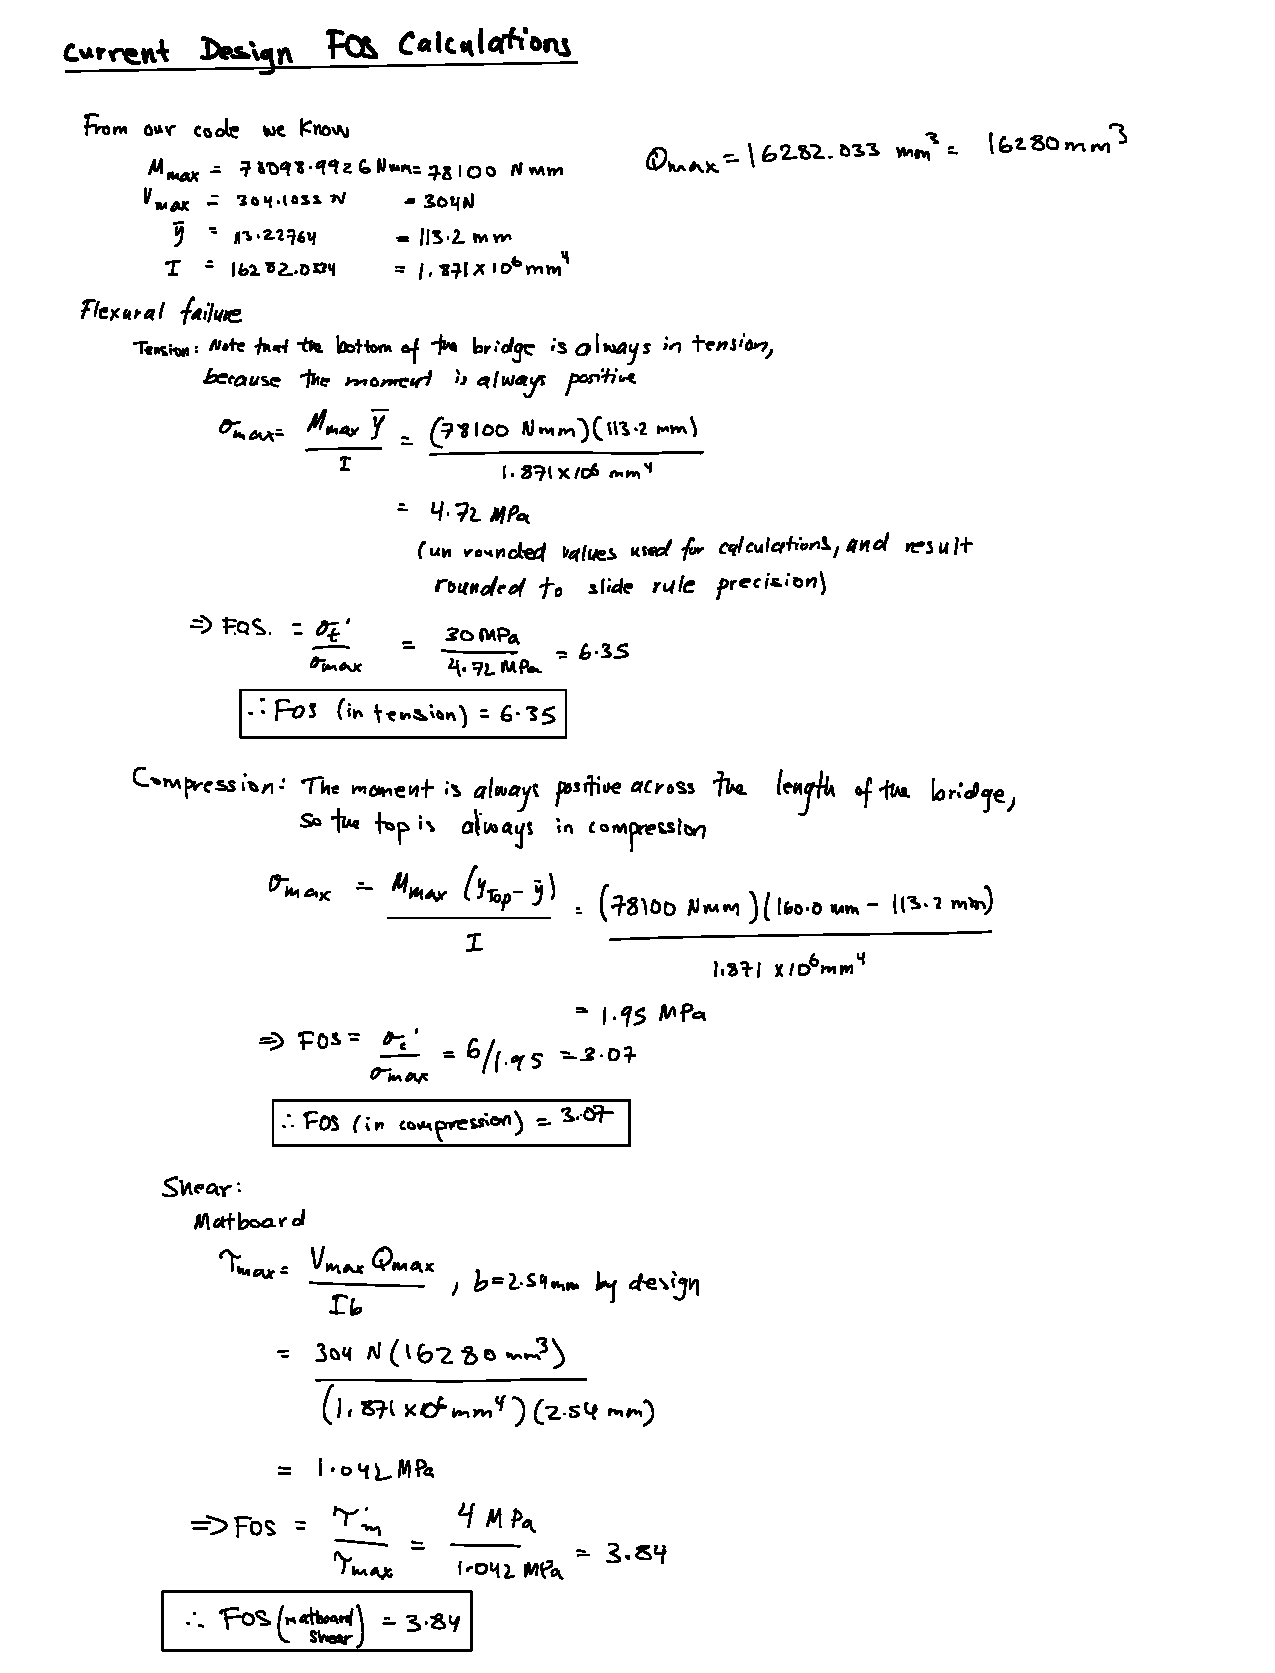
\includepdf[pages=-]{foscurr.pdf}

\section{Evidence of Programming}
\subsection{Design 0 Code and Output}
Below is the code output we used to aid us in our hand calculations for determining the factors of safety against failure, including $\bar{y}$, $I$, $Q_{max}$, and $Q_{glue}$, as well as the SFE and BME, showing both the maximum values the location of the leftmost wheel of the train where they occur. 
\begin{figure}[H]
    \centering
    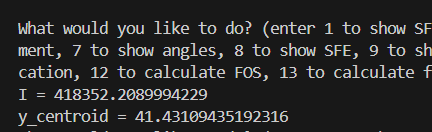
\includegraphics[scale = 0.7]{images/Code DO 1.png}
\end{figure}

\begin{figure}[H]
    \centering
    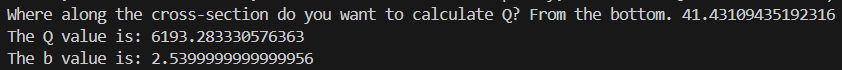
\includegraphics[width=0.95\linewidth]{images/Code D0 2.png}
\end{figure}

\begin{figure}[H]
    \centering
    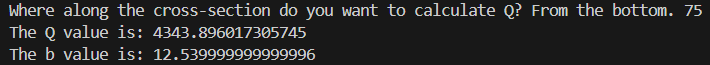
\includegraphics[width=0.95\linewidth]{images/Code D0 3.png}
\end{figure}

\begin{figure}[H]
    \centering
    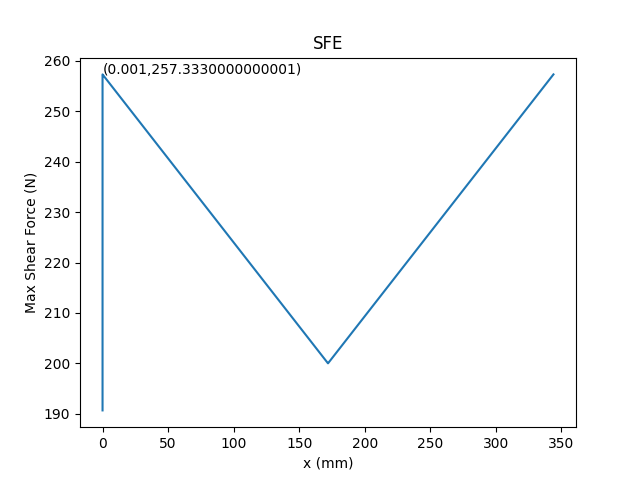
\includegraphics[scale = 0.7]{images/SFE.png}
\end{figure}

\begin{figure}[H]
    \centering
    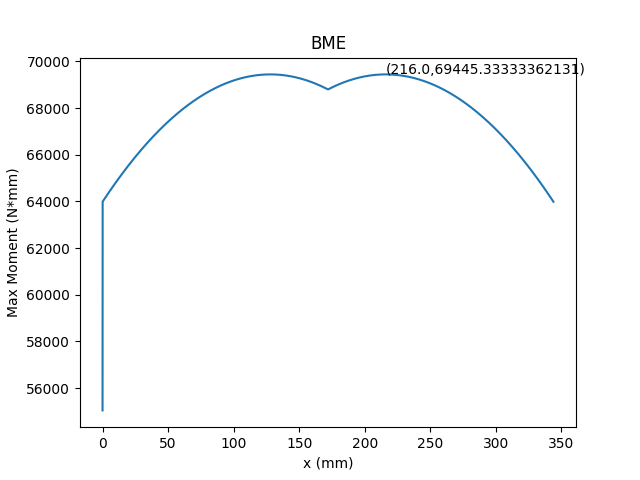
\includegraphics[scale = 0.7]{images/BME.png}
\end{figure}

\subsection{Final Design Code and Output}
Below is the code output we used to aid us in our hand calculations for determining the factors of safety against failure, including $\bar{y}$, $I$, $Q_{max}$, and $Q_{glue}$, as well as the SFE and BME, showing both the maximum values the location of the leftmost wheel of the train where they occur. We also used a graph that illustrated the shear stresses along the cross-section to help as a reference when we calculated our Factor of Safety against shear. Finally, we also used a list of all the different cases of local buckling present in our cross-section, and corresponding stress values for each.
\begin{figure}[H]
    \centering
    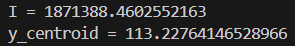
\includegraphics[scale = 0.7]{images/Code F 1.png}
\end{figure}

\begin{figure}[H]
    \centering
    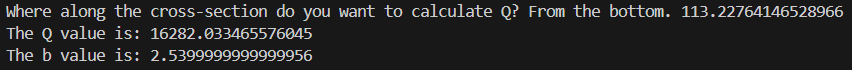
\includegraphics[width=0.95\linewidth]{images/Code F 2.png}
\end{figure}

\begin{figure}[H]
    \centering
    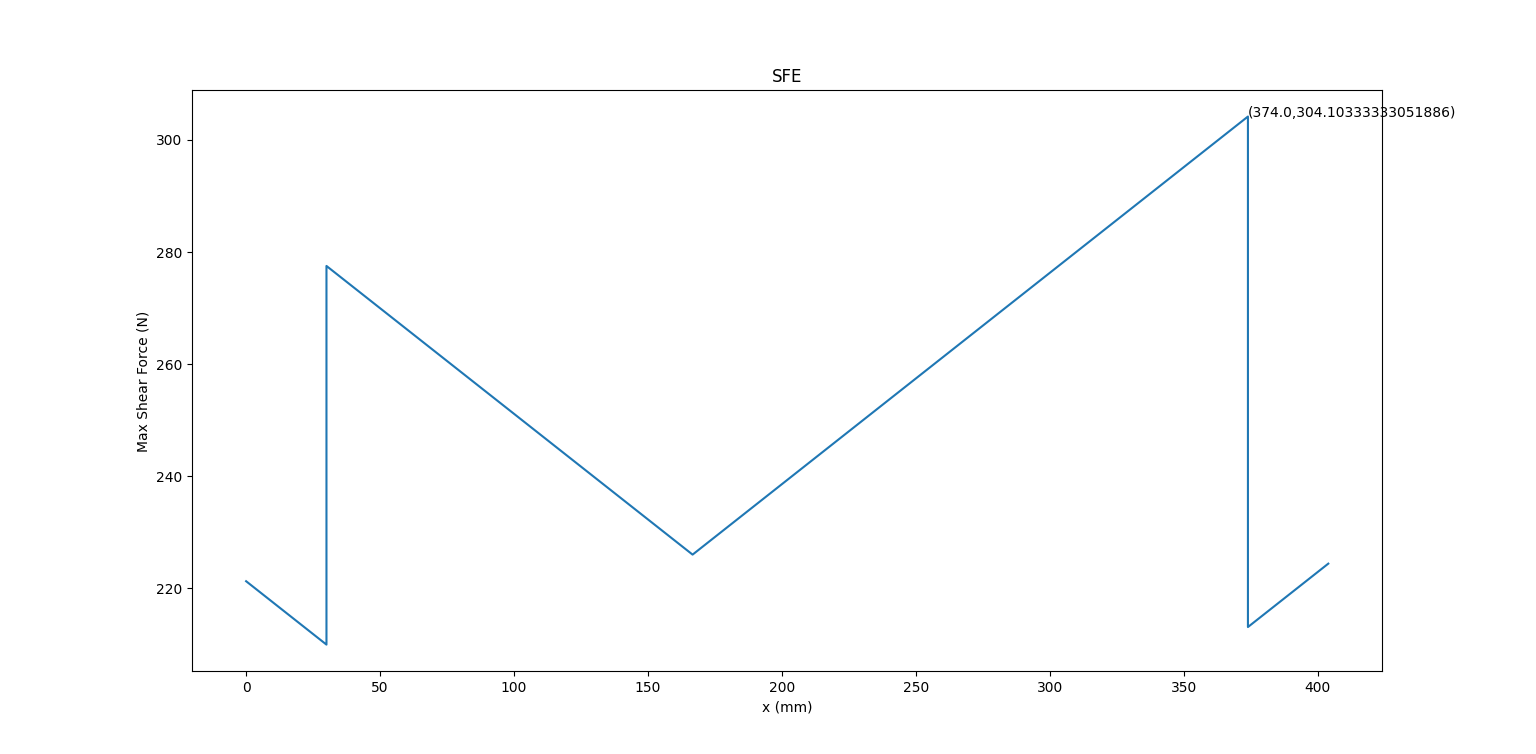
\includegraphics[scale = 0.3]{images/SFE Final.png}
\end{figure}

\begin{figure}[H]
    \centering
    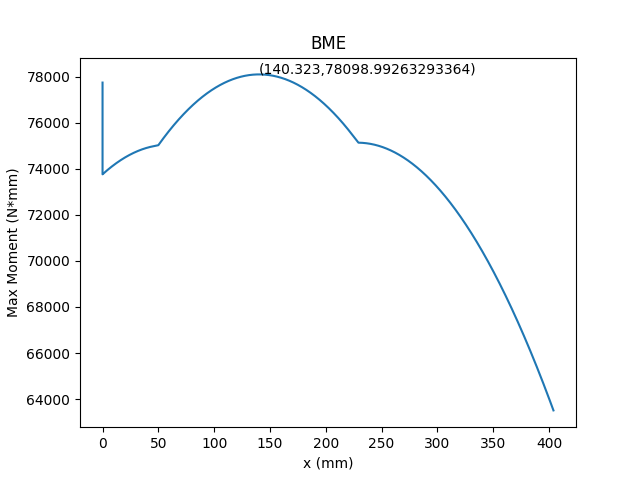
\includegraphics[scale = 0.7]{images/BME Final.png}
\end{figure}

\begin{figure}[H]
    \centering
    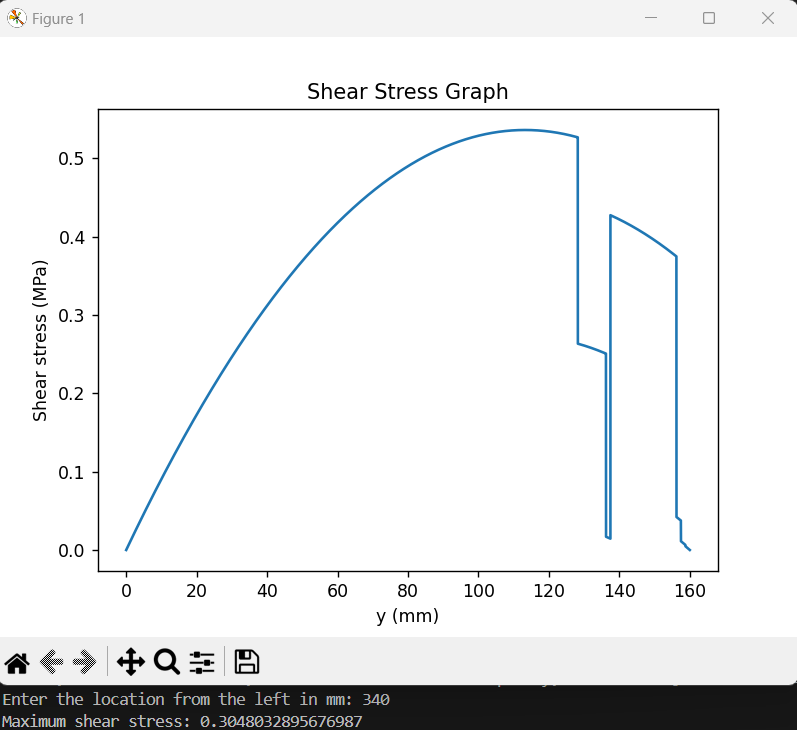
\includegraphics[scale = 0.7]{images/Code F 3.png}
\end{figure}

\begin{figure}[H]
    \centering
    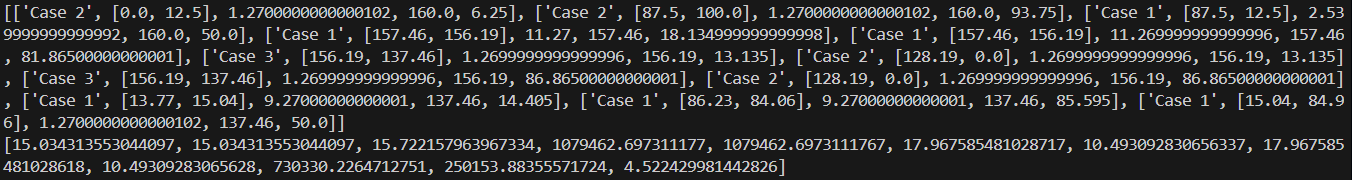
\includegraphics[scale = 0.5]{images/Code F 4.png}
    \caption*{Shown above is our code's output of all the potential local buckling cases present within our cross-section, as well as the critical stress associated with each.}
\end{figure}

\subsection{Explanation of the Code}
\par The Python script we wrote takes in files (see Figures below) describing all the important features of the bridge and loads, and can produce most of the necessary quantities to calculate our Factors of Safety. Outlining the connections between rectangles is needed for the code to determine local buckling cases correctly. Almost all equations used are taken directly from the material taught in CIV102, except for the equations used for shear force and moment. 

\begin{figure}[h]
\begin{minipage}[c]{0.45\linewidth}
\centering
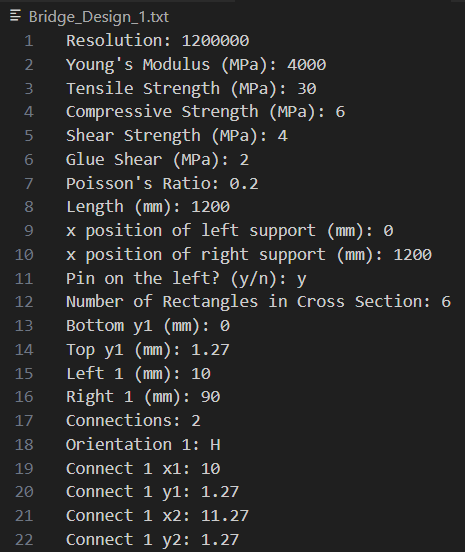
\includegraphics[scale = 0.5]{images/Code File Input Snippet 1.png}
\caption{A snippet of the files we use to input information about the bridge. Rectangles (for the cross-section) are defined using top, bottom, left and right coordinates (in mm).}
\end{minipage}
\hspace{2mm}
\begin{minipage}[c]{0.45\linewidth}
\centering
\vspace{-5.5mm}
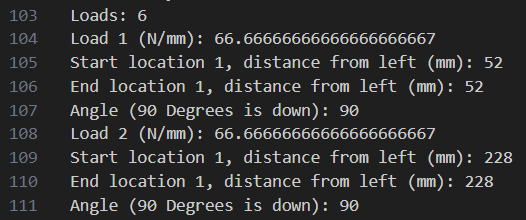
\includegraphics[scale = 0.55]{images/Screenshot 2024-11-25 223050.png}
\caption{A snippet of the input file, describing information about the loads. Loads with the same start and end location are considered as point loads.}
\end{minipage}
\end{figure}

\par Note the use of the Resolution variable. We wanted to use a very high resolution when calculating our shear force and moment, as higher resolutions mean more accurate diagrams and values for the maximum shear and moment attained. For example, a resolution of 1000 means measurements are taken every $1.2 mm$, but a resolution of 1000000 yields a measurement every $1.2 \mu m$. However, using Python to perform numerical integration for the BMD and BME would take minutes, if not hours, for resolutions over 10000. Thus, instead of numerical integration, we solved for shear force and moment analytically and used the code to calculate the required values from our analytical solutions. Since the loading of the bridge only consisted of point/uniformly distributed loads, we knew analytical solutions for shear force and moment existed. 
\pagebreak
\par From CIV102 lectures, we knew that shear force was simply the integral of the applied loads (and reactions), and that the moment was the integral of the shear force. By considering each load's individual contribution to the shear force and moment, and adding the results, it's possible to derive equations for the shear force and moment at any given point from the loading of the bridge. An example of using this process to calculate the BMD is shown below. 
\begin{figure}[h]
\centering
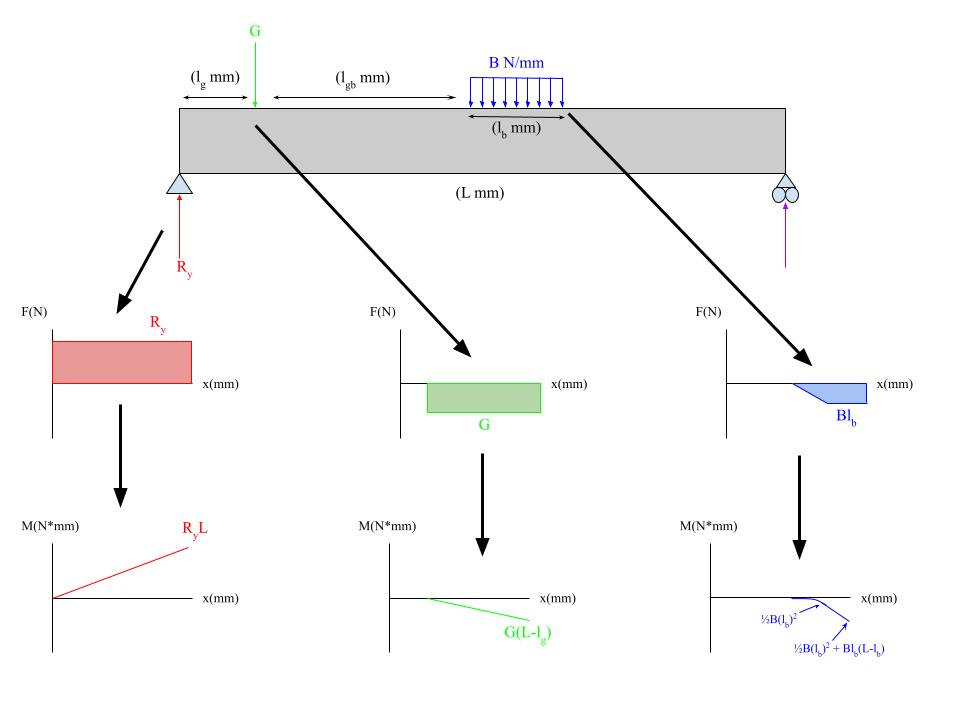
\includegraphics[scale = 0.5]{images/BMD Code Explanation.png}
\caption{A diagram showing how our code separates and analytically determines bending moment from a varying collection of distributed and point loads.}
\end{figure}
\begin{figure}[h]
\centering
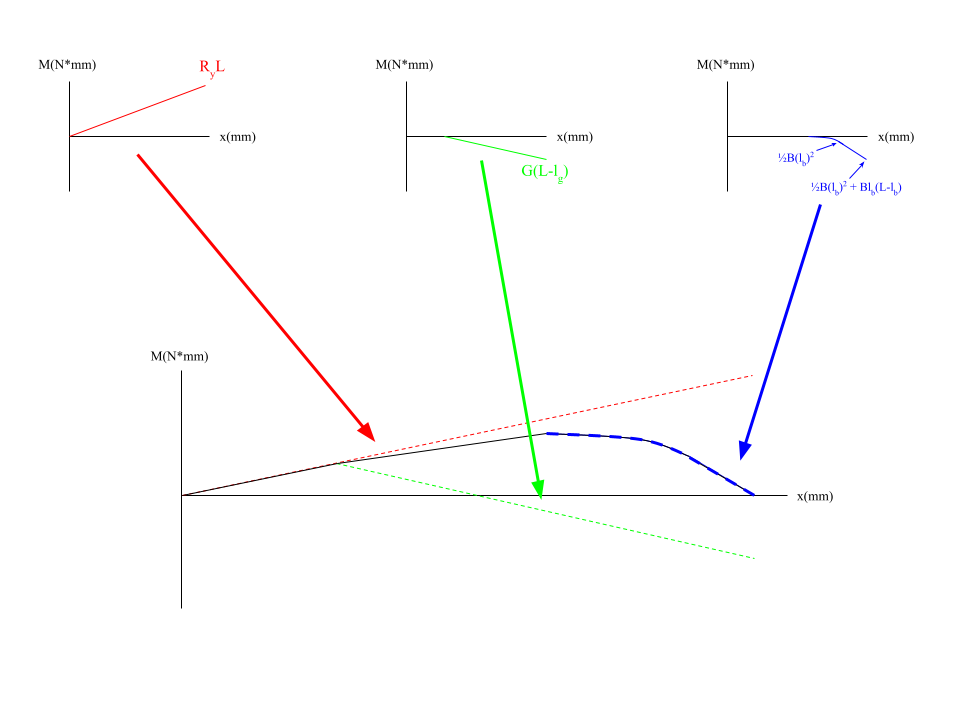
\includegraphics[scale = 0.5]{images/BMD Code Explanation 2.png}
\caption{An illustration of the code combining the results from the previous analysis (Figure 6) to determine the BMD. The black line is the final BMD line.}
\end{figure}
\pagebreak
\par Using this method, we can use resolutions between 1000000 and 10000000 and get results for the SFE / BME in less than a minute. Furthermore, we can apply a similar technique to calculate the exact maximum shear force and moment for the SFD / BMD, regardless of resolution used. Since forces and loading are the only things that change shear, we check shear at the points where the forces change to determine the maximum shear - the maximum shear must be at a location where the forces change from positive to negative, or vice versa. For a similar reason, we also check points where the forces change for the maximum moment - since shear is the derivative of moment, an abrupt change in shear could also result in an abrupt change in whether the moment increases/decreases. However, for moment, we also check points where the shear is 0, as traditionally the maximum/minimum of a graph occurs when its derivative equals 0.
\par 

\section{Link to Code}
All code used can be found \href{https://github.com/epsilon-naut/CIV102-Bridge-Project}{here}. We used the file titled 'TP Buckling Testing.py' for calculations, and other files are old iterations. 

\end{document}